%=========================================
% 	  Technische_Informationen      		 =
%========================================
\chapter{Technische Grundlagen}
In diesem Kapitel werden die Grundlagen erl"autert, die zum Verst"andins der Arbeit notwendig sind.
Zuerst werden die neuronalen Netze bzw. die k"unstlichen neuronalen Netze erkl"art.
Und danach wird erl"autert was Word Embeddings sind.

\section{K"unstliche neuronale Netze}
Der Mensch kann viele verschiedene Aufgaben l"osen, die der Computer jedoch besser und schneller l"osen kann, bis auf Aufgaben die ein hohes Ma"s an Undeterminiertheit, Vagheit und Unsch"arfe aufzeichnen wie fr"uher z.B. Gesicht- oder Spracherkennung. Heutzutage ist es jedoch m"oglich die Sprache oder das Gesicht zu erkennen, wie das Smartphone es uns zeigt. Aber dennoch ist es schwer die Denkweise des Menschen zu imiiteren. Und deswegen wird versucht ein k"unstliches neuronales Netz zu entwickeln, damit die Organisations- und Verarbeitungsprinzipien des menschlichen Gehirns von einem Computer "ubernommen werden k"onnen. Um auch Aufgaben die ein hohes Ma"s an Undeterminiertheit, Vagheit und Unsch"arfe aufzeichnen, besser und schneller bew"altigt werden k"onnen. Aber was genau ist ein k"unstliches neuronales Netz? 
Ein k"unstlich neuronales Netz kann man sich wie ein Graph mit Knoten und Kanten, die gewichtet und gerichtet sind, vorstellen. Die Knoten sind in Schichten unterteilt, je mehr Knoten hintereinander kommen desto mehr Schichten wird es geben. Es gibt am Anfang des Graphen eine Eingabeschicht und am Ende eine Ausgabeschicht. Die Menge der Knoten in den Schichten sind, ist beliebig gro"s. Die Schichten die zwischen Ein- und Ausgabeschicht werden verdeckte, versteckte oder verborgene Schicht genannt. Die Knoten verarbeiten eine beliebige Anzahl numerischer  Eingangswerte und  erzeugen  einen  numerischen Ausgabewert. Eingangswerte  sind  entweder  Ausgabewerte  anderer Knoten oder Eingabemuster aus der Systemumgebung, also der netzwerkexternen Umwelt.\\
\begin{figure}[bth]
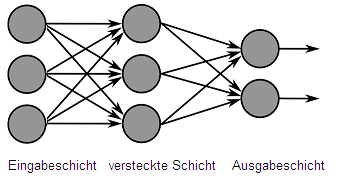
\includegraphics{Graphics/neuronales_netz.png}
\caption[Neuronales Netzwerk]{Aufbau eines Neuronales Netzwerk  \cite{todesco:2018}}
\end{figure}\\
%Quelle des Bildes: https://www.hyperkommunikation.ch/lexikon/neuronales_netz.htm
\textit{"K"unstliche Neuronale Netze weisen Kernkomponenten oder Grundbausteine auf, die sich in allen Netzwerktypen wiederfinden. Die statischen Kernkomponenten geben  \acs{KNN} die r"aumliche Gestalt bzw. Struktur."}
\cite{Strecker97}


\section{Word Embeddings}
Ein Algorithmus des Word Embeddings ist der sogenannte word2Vec-Algorithmus. Dieser Algorithmus ist ein un"uberwachter Lernalgorithmus, mit ihm kann man die Beziehungen der W"orter erkennen und sie in "Ahnlichkeits-Cluster unterteilen.\\
\textit{"Durch eine clevere Verwendung von Vektorr"aumen ist das Modell dann in der Lage, bestimmte W"orter durch einfache Vektorberechnungen nachzubilden, beispielsweise Knecht - Mann + Frau = Magd."}
\cite{raschka:2017}
\begin{figure}[bth]
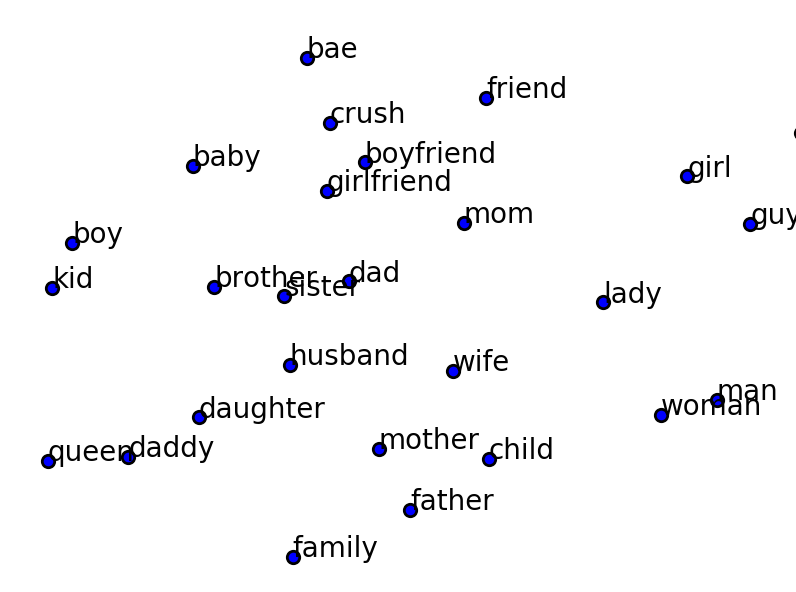
\includegraphics[width=15cm]{Graphics/cluster.png}\caption["Ahnlichkeits-Cluster]{Darstellung eines "Ahnlichkeits-Cluster  \cite{marivate:2017}}
\end{figure}

Wie man im Bild sehen kann, sind die W"orter deren Bedeutung "ahnlich sind nahe beieinander. Auch wenn es nicht immer mit allen W"ortern richtig ist. 

%Quelle des Buches: Machine Learning mit Python 
% Quelle: http://geb.uni-giessen.de/geb/volltexte/2004/1697/pdf/Apap_WI_1997_10.pdf
\pagebreak
\section{Zusammenhang von Word Embeddings und \acs{KNN}}
Word2vec benutzt Modelle, die verwendet werden um Word Embeddings zu erstellen. Diese Modelle sind flache und beliebig-schichtige neuronale Netze, die darauf trainiert sind, sprachliche Kontexte von W"ortern zu rekonstruieren. Als Eingabe wird eine gro"ser Korpus von Texten benutzt, daraus wird ein Vektorraum erzeugt, der typischerweise aus mehreren hundert Dimensionen besteht, wobei jedem eindeutigen Wort im Korpus ein entsprechender Vektor im Raum zugeordnet wird. Wortvektoren werden in dem Vektorraum positioniert, so dass W"orter, die gemeinsame Kontexte in dem Korpus teilen, in dem Raum nahe beieinander angeordnet sind.